
\section*{CHƯƠNG 1. THU THẬP YÊU CẦU}
\setcounter{section}{1}
\setcounter{subsection}{0} %LƯU Ý MỖI LẦN THÊM CHƯƠNG MỚI CẦN THÊM CÂU NÀY ĐỂ RESET THỨ TỰ CỦA SUBSECTON VỀ 1
\setcounter{table}{0} % LƯU Ý SAU MỖI LẦN GỌI BẢNG HAY HÌNH ẢNH PHẢI THÊM CÂU NÀY ĐỂ RESET THỨ TỰ
\setcounter{figure}{0} %% LƯU Ý SAU MỖI LẦN GỌI BẢNG HAY HÌNH ẢNH PHẢI THÊM CÂU NÀY ĐỂ RESET THỨ TỰ
\addcontentsline{toc}{section}{\numberline{}CHƯƠNG 1. THU THẬP YÊU CẦU}
Chương này sẽ tiến hành thu thập yêu cầu cho dự án đề tài "Hệ thống quản lý dữ liệu điện tim và tương tác giữa bênh nhân - bác sĩ"
dựa trên các mục tiêu đã nêu ra trong Mục Đề xuất hệ thống ở Phần mở đầu.

\subsection{Phân tích yêu cầu hệ thống}
\subsubsection{Yêu cầu chức năng của hệ thống}
Hệ thống được xây dựng để đáp ứng nhu cầu riêng của từng nhóm người dùng, mang đến các tính năng giúp đơn giản hóa quy trình thu thập, xử lý và lưu trữ dữ liệu y tế. Đồng thời, hệ thống còn đóng vai trò là cầu nối, tăng cường sự tương tác hiệu quả giữa bệnh nhân và bác sĩ, góp phần nâng cao trải nghiệm người dùng và chất lượng chăm sóc sức khỏe. Các chức năng chính bao gồm:
\begin{adjustwidth}{1.5em}{}
	\begin{itemize}
		\item Ghi dữ liệu đo từ thiết bị: Ứng dụng trên điện thoại thu nhận dữ liệu đo điện tim từ thiết bị thông qua kết nối Bluetooth.
		      Dữ liệu này được lưu trữ dưới dạng file định dạng .csv và đồng bộ trực tiếp lên máy chủ hệ thống, đảm bảo an toàn và sẵn sàng cho việc truy cập, phân tích sau này.
		\item Hiển thị dữ liệu: Các số liệu được lưu trữ trên máy chủ sẽ được xử lý và tính toán theo các công thức chuyên môn, sau đó được hiển thị trực quan trên website và ứng dụng di động dưới dạng đồ thị đường, giúp bác sĩ dễ dàng theo dõi và phân tích các chỉ số sức khỏe.
		\item Lưu trữ dữ liệu: Hệ thống hỗ trợ lưu trữ dữ liệu đo điện tim từ thiết bị trên cả ứng dụng di động và máy chủ trung tâm. Dữ liệu được đồng bộ hóa tự động từ ứng dụng lên máy chủ, đảm bảo an toàn và bảo mật tuyệt đối. Việc lưu trữ song song này giúp bảo vệ dữ liệu quan trọng, đảm bảo tính toàn vẹn và khả năng truy cập cho mục đích phân tích hoặc sử dụng trong tương lai, mang lại sự tin cậy cao cho người dùng.
		\item Trao đổi và chia sẻ thông tin về dữ liệu y tế: Hệ thống giúp người dùng có thể trao đổi trực tiếp với bác sĩ, chia sẻ kết quả đo điện tim, hỏi đáp về các vấn đề sức khỏe và các vấn đề liên quan đến thiết bị. Ngoài ra, hệ thống còn hỗ trợ người dùng đặt lịch khám trực tiếp với bác sĩ, mang lại sự tiện lợi và hỗ trợ đáng kể cho người dùng trong việc xác định tình trạng sức khoẻ hiện tại và nhận được sự tư vấn kịp thời.
	\end{itemize}
\end{adjustwidth}
\textbf{Đối với bệnh nhân:}
\begin{adjustwidth}{1.5em}{}
	\begin{itemize}
		\item Đăng nhập và đăng ký tài khoản bằng thông tin cá nhân, bao gồm tên, địa chỉ email, ngày sinh, số điện thoại và mật khẩu.
		\item Cập nhật các thông tin cá nhân.
		\item Được theo dõi điện tim trực tiếp khi kết nối ứng dụng di động với thiết bị đo điện tim thông qua Bluetooth.
		\item Xem kết quả các phiên đo của mình, bao gồm biểu đồ và các thông số liên quan.
		\item Nhận thông báo và có thể trao đổi trực tiếp với bác sĩ về tình hình sức khoẻ và các kết quả đo được từ thiết bị thông qua đặt lịch khám hoặc tin nhắn trực tiếp.
	\end{itemize}
\end{adjustwidth}
\textbf{Đối với bác sĩ:}
\begin{adjustwidth}{1.5em}{}
	\begin{itemize}
		\item Đăng nhập và đăng ký tài khoản bằng thông tin cá nhân, bao gồm tên, địa chỉ email, ngày sinh, số điện thoại và mật khẩu.
		\item Cập nhật thông tin cá nhân.
		\item Quản lý danh sách lịch hẹn, chấp nhận hoặc từ chối lịch hẹn đã đặt của bệnh nhân.
		\item Quản lý danh sách bệnh nhân đã được chấp nhận lịch hẹn.
		\item Quản lý danh sách các bản ghi dữ liệu đo của các bệnh nhân đã đặt lịch hẹn thành công.
		\item Nhận thông báo và có thể trao đổi trực tiếp với bệnh nhân về tình hình sức khoẻ và các kết quả đo được từ thiết bị.
	\end{itemize}
\end{adjustwidth}
\textbf{Đối với quản trị viên:}
\begin{adjustwidth}{1.5em}{}
	\begin{itemize}
		\item Đăng nhập và đăng ký tài khoản bằng thông tin cá nhân, bao gồm tên, địa chỉ email, số điện thoại và mật khẩu.
		\item Cập nhật thông tin cá nhân.
		\item Quản lý danh sách người dùng trong hệ thống, bao gồm bệnh nhân và bác sĩ.
		\item Quản lý danh sách thiết bị, chịu trách nhiệm phân công thiết bị cho người dùng.
		\item Quản lý các bản ghi đã đo được.
		\item Quản lý lịch hẹn của toàn bộ người dùng.
	\end{itemize}
\end{adjustwidth}

\subsubsection{Yêu cầu phi chức năng của hệ thống}
\begin{itemize}
	\item Hệ thống có thể tương thích với hầu hết các trình duyệt phổ biến hiện nay.
	\item Hệ thống đảm bảo tính bảo mật và quyền riêng tư thông tin của người dùng.
	\item Hệ thống phải có giao diện người dùng thân thiện, dễ sử dụng để có thể tương tác mà không gặp quá nhiều khó khăn.
	\item Thời gian phản hồi của hệ thống phải nhanh chóng và ổn định.
	\item Hệ thống cần được tối ưu hóa để hoạt động hiệu quả ngay cả khi có lưu lượng truy cập cao.
	\item Hệ thống cần được sao lưu dữ liệu định kỳ để đảm bảo tính an toàn và khả năng khôi phục dữ liệu khi cần thiết.
\end{itemize}

\subsubsection{Yêu cầu về người dùng hệ thống}
Hệ thống được thiết kế để phục vụ các đối tượng sau:
\begin{adjustwidth}{1.5em}{}
	\begin{itemize}
		\item Bệnh nhân: Sử dụng hệ thống để theo dõi dữ liệu điện tim của mình thông qua website.
		      Bệnh nhân có thể đăng nhập vào tài khoản để truy cập thông tin cá nhân, xem danh sách bác sĩ, thông tin các bản ghi điện tim đã đo, đồng thời tìm kiếm và chọn lịch hẹn phù hợp để đăng ký.
		      Ngoài ra, hệ thống còn cung cấp tính năng nhắn tin trực tiếp, giúp bệnh nhân dễ dàng trao đổi và nhận tư vấn từ bác sĩ.

		\item Bác sĩ: Hệ thống hỗ trợ bác sĩ quản lý và theo dõi tình trạng sức khỏe của các bệnh nhân đã đặt lịch hẹn thành công.
		      Bác sĩ được phép truy cập kết quả các phiên đo, cung cấp tư vấn, trao đổi thông tin y tế, và chủ động đặt lịch tái khám khi cần.
		      Ngoài ra, bác sĩ có thể tương tác với bệnh nhân qua tính năng nhắn tin hoặc nhóm chat để thảo luận và chia sẻ thông tin chuyên môn.

		\item Quản trị viên: Quản trị viên chịu trách nhiệm quản lý thông tin tài khoản của bệnh nhân, bác sĩ và các thiết bị y tế, đồng thời giám sát lịch khám và dữ liệu đo lường.
		      Họ đảm bảo hệ thống vận hành chính xác, hiệu quả và đáp ứng nhu cầu của mọi người dùng.
	\end{itemize}
\end{adjustwidth}

Quá trình phân tích yêu cầu hệ thống đóng vai trò quan trọng trong việc xác định cụ thể các chức năng, yêu cầu phi chức năng, và các nhóm đối tượng người dùng mà hệ thống hướng tới phục vụ.
Từ cơ sở này, việc thiết kế và phát triển hệ thống quản lý dữ liệu điện tim và tương tác giữa bệnh nhân và bác sĩ được triển khai, đảm bảo đáp ứng đầy đủ nhu cầu của người dùng,
đồng thời tối ưu hóa về hiệu suất, bảo mật và khả năng sử dụng của hệ thống.

\subsection{Sơ đồ các trường hợp sử dụng}

\subsubsection{Sơ đồ tổng quát các trường hợp sử dụng}

\begin{figure}[H]
	\centering
	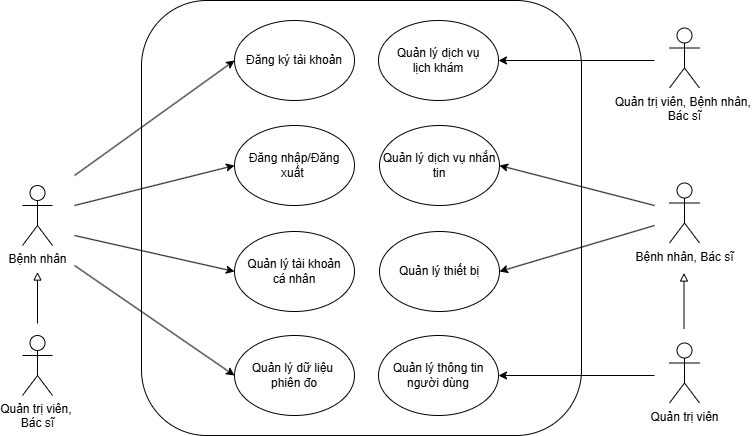
\includegraphics[width=16cm,height=11cm]{Images/use_case/use_case_general.png}
	\caption[Sơ đồ tổng quát các trường hợp sử dụng của hệ thống]{\bfseries \fontsize{12pt}{0pt}
		\selectfont Sơ đồ tổng quát các trường hợp sử dụng}
	\label{use_case_general} %đặt tên cho ảnh
\end{figure}

\subsubsection{Sơ đồ trường hợp sử dụng chức năng tạo tài khoản người dùng}

\begin{figure}[H]
	\centering
	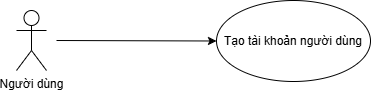
\includegraphics[width=9cm,height=2.5cm]{Images/use_case/use_case_register.png}
	\caption[Sơ đồ trường hợp sử dụng chức năng tạo tài khoản người dùng]{\bfseries \fontsize{12pt}{0pt}
		\selectfont Sơ đồ trường hợp sử dụng chức năng tạo tài khoản người dùng}
	\label{use_case_register} %đặt tên cho ảnh
\end{figure}

\begin{table}[H]
	\caption{\bfseries \fontsize{12pt}{0pt}\selectfont Phân tích trường hợp sử dụng chức năng tạo tài khoản người dùng}
	\centering
	\begin{tabularx}{\textwidth}{|X|X|}
		\hline
		\textbf{Tên chức năng} & \textbf{Tạo tài khoản người dùng}                                                           \\
		\hline
		Tác nhân               & Người sử dụng hệ thống (Bệnh nhân, Bác sĩ, Quản trị viên)                                   \\
		\hline
		Mô tả                  & Hỗ trợ người dùng tạo tài khoản mới để truy cập các tính năng và dịch vụ của hệ thống       \\
		\hline
		Điều kiện trước        & Người dùng cần sử dụng thiết bị hỗ trợ kết nối Internet và chưa có tài khoản trong hệ thống \\
		\hline
		Dòng sự kiện chính     &
		- Người dùng truy cập màn hình tạo tài khoản mới \newline
		- Nhập các thông tin cần thiết như email, mật khẩu và thông tin cá nhân \newline
		- Hệ thống kiểm tra tính hợp lệ của thông tin được cung cấp \newline
		- Nếu thông tin hợp lệ, tài khoản sẽ được tạo và thông báo thành công. Ngược lại, hệ thống hiển thị lỗi và yêu cầu người dùng nhập lại \newline
		- Hoàn thành quá trình tạo tài khoản người dùng                                                                      \\
		\hline
	\end{tabularx}
\end{table}

\subsubsection{Sơ đồ trường hợp sử dụng chức năng đăng nhập và đăng xuất khỏi hệ thống}

\begin{figure}[H]
	\centering
	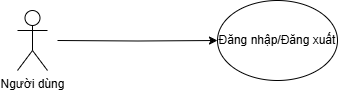
\includegraphics[width=9cm,height=2.5cm]{Images/use_case/use_case_login_logout.png}
	\caption[Sơ đồ trường hợp sử dụng chức năng đăng nhập và đăng xuất khỏi hệ thống]{\bfseries \fontsize{12pt}{0pt}
		\selectfont Sơ đồ trường hợp sử dụng chức năng đăng nhập và đăng xuất khỏi hệ thống}
	\label{use_case_login_logout} %đặt tên cho ảnh
\end{figure}

\begin{table}[H]
	\caption{\bfseries \fontsize{12pt}{0pt}\selectfont Phân tích trường hợp sử dụng chức năng đăng nhập/đăng xuất}
	\centering
	\begin{tabularx}{0.9\textwidth}{|c|X|}
		\hline
		\textbf{Tên chức năng} & \textbf{Đăng nhập và đăng xuất hệ thống}                                                                                    \\
		\hline
		Tác nhân               & Người sử dụng hệ thống                                                                                                      \\
		\hline
		Mô tả                  & Cung cấp khả năng cho người dùng truy cập vào hệ thống bằng tài khoản đã đăng ký và rời khỏi hệ thống khi không cần sử dụng \\
		\hline
		Điều kiện trước        & Người dùng phải có tài khoản hợp lệ                                                                                         \\
		\hline
		Dòng sự kiện chính     &
		Đăng nhập: \newline
		- Người dùng chọn tùy chọn đăng nhập \newline
		- Nhập email và mật khẩu vào biểu mẫu \newline
		- Hệ thống kiểm tra tính hợp lệ và xác thực tài khoản \newline
		- Nếu thông tin hợp lệ, hệ thống cho phép truy cập và hiển thị trang chủ. Nếu không, hiển thị lỗi yêu cầu nhập lại tài khoản\newline
		- Hoàn thành quá trình đăng nhập \newline
		Đăng xuất: \newline
		- Người dùng chọn tùy chọn đăng xuất \newline
		- Hệ thống hủy phiên làm việc và đưa người dùng về giao diện đăng nhập  \newline
		- Hoàn thành quá trình đăng xuất                                                                                                                     \\
		\hline
	\end{tabularx}
\end{table}

\subsubsection{Sơ đồ trường hợp sử dụng chức năng quản lý tài khoản người dùng}

\begin{figure}[H]
	\centering
	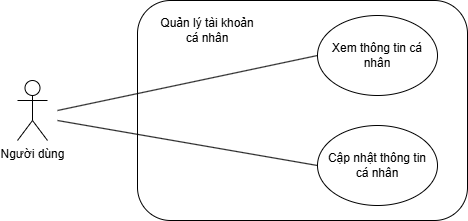
\includegraphics[width=12cm,height=6cm]{Images/use_case/use_case_account_info.png}
	\caption[Sơ đồ trường hợp sử dụng chức năng quản lý tài khoản người dùng]{\bfseries \fontsize{12pt}{0pt}
		\selectfont Sơ đồ trường hợp sử dụng chức năng quản lý tài khoản người dùng}
	\label{use_case_account_info} %đặt tên cho ảnh
\end{figure}

\begin{table}[H]
	\caption{\bfseries \fontsize{12pt}{0pt}\selectfont Phân tích trường hợp sử dụng chức năng quản lý tài khoản người dùng}
	\centering
	\begin{tabularx}{0.9\textwidth}{|c|X|}
		\hline
		\textbf{Tên chức năng} & \textbf{Quản lý thông tin tài khoản người dùng}                                  \\
		\hline
		Tác nhân               & Người sử dụng hệ thống                                                           \\
		\hline
		Mô tả                  & Hỗ trợ người dùng xem và chỉnh sửa các thông tin cá nhân được lưu trong hệ thống \\
		\hline
		Điều kiện trước        & Người dùng cần đăng nhập vào hệ thống                                            \\
		\hline
		Dòng sự kiện chính     &
		- Người dùng truy cập tính năng quản lý thông tin cá nhân \newline
		- Hệ thống hiển thị các thông tin hiện tại của tài khoản \newline
		- Người dùng thực hiện thay đổi thông tin cá nhân khi cần \newline
		- Hệ thống kiểm tra tính chính xác và hợp lệ của thông tin đã cập nhật \newline
		- Nếu thông tin hợp lệ, hệ thống tiến hành cập nhật và hiển thị thông báo. Nếu không, hiển thị lỗi và yêu cầu nhập lại \newline
		- Hoàn thành quá trình quản lý thông tin tài khoản cá nhân                                                \\
		\hline
	\end{tabularx}
\end{table}

\subsubsection{Sơ đồ trường hợp sử dụng chức năng quản lý người dùng hệ thống}

\begin{figure}[H]
	\centering
	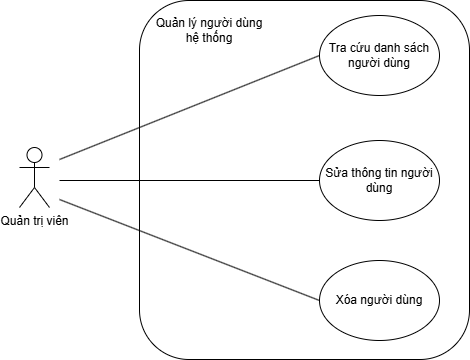
\includegraphics[width=12cm,height=12cm]{Images/use_case/use_case_user.png}
	\caption[Sơ đồ trường hợp sử dụng chức năng quản lý người dùng]{\bfseries \fontsize{12pt}{0pt}
		\selectfont Sơ đồ trường hợp sử dụng chức năng quản lý người dùng hệ thống}
	\label{use_case_user} %đặt tên cho ảnh
\end{figure}

\begin{table}[H]
	\caption{\bfseries \fontsize{12pt}{0pt}\selectfont Phân tích trường hợp sử dụng chức năng tra cứu danh sách người dùng}
	\centering
	\begin{tabularx}{0.9\textwidth}{|c|X|}
		\hline
		\textbf{Tên chức năng} & \textbf{Tra cứu danh sách người dùng}                                                                             \\
		\hline
		Tác nhân               & Quản trị viên                                                                                                     \\
		\hline
		Mô tả                  & Hỗ trợ quản trị viên thực hiện các tác vụ như tra cứu và quản lý thông tin chi tiết của người dùng trong hệ thống \\
		\hline
		Điều kiện trước        & Quản trị viên phải đăng nhập vào hệ thống với quyền truy cập hợp lệ                                               \\
		\hline
		Dòng sự kiện chính     &
		- Quản trị viên truy cập tính năng tra cứu danh sách người dùng \newline
		- Hệ thống hiển thị danh sách thông tin tất cả người dùng trong hệ thống \newline
		- Quản trị viên thực hiện tìm kiếm và chọn một người dùng cụ thể \newline
		- Hệ thống cung cấp thông tin chi tiết của người dùng được chọn \newline
		- Hoàn thành quá trình tra cứu danh sách người dùng                                                                                        \\
		\hline
	\end{tabularx}
\end{table}

\begin{table}[H]
	\caption{\bfseries \fontsize{12pt}{0pt}\selectfont Phân tích trường hợp sử dụng chức năng tra cứu danh sách bác sĩ}
	\centering
	\begin{tabularx}{0.9\textwidth}{|c|X|}
		\hline
		\textbf{Tên chức năng} & \textbf{Tra cứu danh sách bác sĩ}                                         \\
		\hline
		Tác nhân               & Bệnh nhân                                                                 \\
		\hline
		Mô tả                  & Hỗ trợ bệnh nhân tra cứu thông tin chi tiết của các bác sĩ trong hệ thống \\
		\hline
		Điều kiện trước        & Bệnh nhân phải đăng nhập vào hệ thống với quyền truy cập hợp lệ           \\
		\hline
		Dòng sự kiện chính     &
		- Bệnh nhân truy cập tính năng tra cứu danh sách bác sĩ \newline
		- Hệ thống hiển thị danh sách các bác sĩ cùng thông tin cơ bản. \newline
		- Bệnh nhân chọn bác sĩ cụ thể từ danh sách. \newline
		- Hệ thống hiển thị thông tin chi tiết về bác sĩ được chọn. \newline
		- Hoàn thành quá trình tra cứu danh sách bác sĩ trong hệ thống                                     \\
		\hline
	\end{tabularx}
\end{table}

\begin{table}[H]
	\caption{\bfseries \fontsize{12pt}{0pt}\selectfont Phân tích trường hợp sử dụng chức năng tra cứu danh sách bệnh nhân}
	\centering
	\begin{tabularx}{0.9\textwidth}{|c|X|}
		\hline
		\textbf{Tên chức năng} & \textbf{Tra cứu danh sách bệnh nhân đang theo dõi}                                                      \\
		\hline
		Tác nhân               & Bác sĩ                                                                                                  \\
		\hline
		Mô tả                  & Hỗ trợ bác sĩ tìm kiếm và xem thông tin chi tiết của các bệnh nhân mà họ đang phụ trách trong hệ thống. \\
		\hline
		Điều kiện trước        & Bác sĩ phải đăng nhập vào hệ thống với quyền truy cập hợp lệ                                            \\
		\hline
		Dòng sự kiện chính     &
		- Bác sĩ truy cập tính năng tra cứu danh sách bệnh nhân đang phụ trách \newline
		- Hệ thống hiển thị danh sách các bệnh nhân cùng thông tin cơ bản. \newline
		- Bác sĩ chọn bệnh nhân cụ thể từ danh sách. \newline
		- Hệ thống cung cấp thông tin chi tiết của bệnh nhân được chọn. \newline
		- Hoàn thành quá trình tra cứu danh sách bệnh nhân                                                                               \\
		\hline
	\end{tabularx}
\end{table}

\begin{table}[H]
	\caption{\bfseries \fontsize{12pt}{0pt}\selectfont Phân tích trường hợp sử dụng chức năng tra cứu danh sách người dùng}
	\centering
	\begin{tabularx}{0.9\textwidth}{|c|X|}
		\hline
		\textbf{Tên chức năng} & \textbf{Tra cứu danh sách người dùng}                                                                             \\
		\hline
		Tác nhân               & Quản trị viên                                                                                                     \\
		\hline
		Mô tả                  & Hỗ trợ quản trị viên thực hiện các tác vụ như tra cứu và quản lý thông tin chi tiết của người dùng trong hệ thống \\
		\hline
		Điều kiện trước        & Quản trị viên phải đăng nhập vào hệ thống với quyền truy cập hợp lệ                                               \\
		\hline
		Dòng sự kiện chính     &
		- Quản trị viên truy cập tính năng quản lý danh sách người dùng \newline
		- Hệ thống hiển thị danh sách thông tin tất cả người dùng trong hệ thống \newline
		- Quản trị viên thực hiện tìm kiếm và chọn một người dùng cụ thể \newline
		- Hệ thống cung cấp thông tin chi tiết của người dùng được chọn \newline
		- Hoàn thành quá trình tra cứu danh sách người dùng                                                                                        \\
		\hline
	\end{tabularx}
\end{table}

\begin{table}[H]
	\caption{\bfseries \fontsize{12pt}{0pt}\selectfont Phân tích trường hợp sử dụng chức năng chỉnh sửa thông tin người dùng}
	\centering
	\begin{tabularx}{0.9\textwidth}{|c|X|}
		\hline
		\textbf{Tên chức năng} & \textbf{Chỉnh sửa thông tin người dùng}                                                                                                               \\
		\hline
		Tác nhân               & Quản trị viên                                                                                                                                         \\
		\hline
		Mô tả                  & Hỗ trợ quản trị viên thực hiện việc chỉnh sửa thông tin chi tiết của người dùng trong hệ thống, đảm bảo thông tin được cập nhật chính xác và kịp thời \\
		\hline
		Điều kiện trước        & Quản trị viên phải đăng nhập vào hệ thống với quyền truy cập hợp lệ                                                                                   \\
		\hline
		Dòng sự kiện chính     &
		- Quản trị viên truy cập chức năng chỉnh sửa thông tin người dùng \newline
		- Hệ thống hiển thị thông tin hiện tại của người dùng \newline
		- Quản trị viên nhập thông tin cần chỉnh sửa \newline
		- Hệ thống kiểm tra tính hợp lệ của thông tin mới \newline
		- Nếu thông tin hợp lệ, hệ thống cập nhật thông tin và gửi thông báo thành công \newline
		- Nếu thông tin không hợp lệ, hệ thống hiển thị lỗi và yêu cầu chỉnh sửa lại    \newline
		- Hoàn thành quá trình chỉnh sửa thông tin người dùng                                                                                                                          \\
		\hline
	\end{tabularx}
\end{table}

\begin{table}[H]
	\caption{\bfseries \fontsize{12pt}{0pt}\selectfont Phân tích trường hợp sử dụng chức năng xóa người dùng khỏi hệ thống}
	\centering
	\begin{tabularx}{0.9\textwidth}{|c|X|}
		\hline
		\textbf{Tên chức năng} & \textbf{Xóa người dùng}                                                              \\
		\hline
		Tác nhân               & Quản trị viên                                                                        \\
		\hline
		Mô tả                  & Hỗ trợ quản trị viên thực hiện việc xóa người dùng không còn hoạt động khỏi hệ thống \\
		\hline
		Điều kiện trước        & Quản trị viên phải đăng nhập vào hệ thống với quyền truy cập hợp lệ                  \\
		\hline
		Dòng sự kiện chính     &
		- Hệ thống hiển thị danh sách người dùng hiện có \newline
		- Quản trị viên chọn các người dùng cần xóa khỏi hệ thống\newline
		- Hệ thống hiển thị yêu cầu xác nhận xóa \newline
		- Quản trị viên xác nhận hành động xóa \newline
		- Hệ thống xóa người dùng được chọn và cập nhật dữ liệu đồng thời gửi thông báo xóa thành công \newline
		- Hoàn thành quá trình xóa người dùng khỏi hệ thống                                                           \\
		\hline
	\end{tabularx}
\end{table}

\subsubsection{Sơ đồ trường hợp sử dụng chức năng quản lý thiết bị y tế}

\begin{figure}[H]
	\centering
	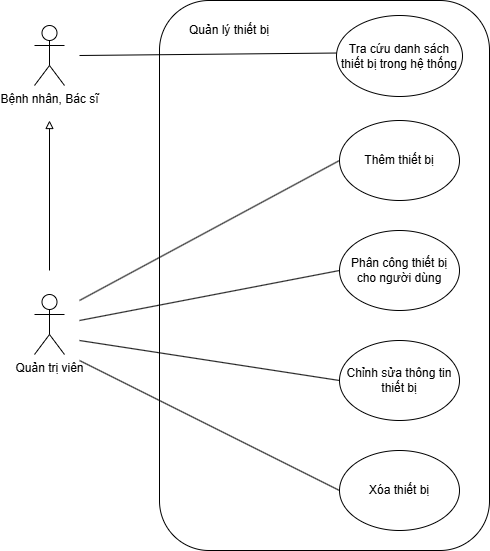
\includegraphics[width=12cm,height=11.5cm]{Images/use_case/use_case_device.png}
	\caption[Sơ đồ trường hợp sử dụng chức năng quản lý thiết bị y tế]{\bfseries \fontsize{12pt}{0pt}
		\selectfont Sơ đồ trường hợp sử dụng chức năng quản lý thiết bị y tế}
	\label{use_case_device} %đặt tên cho ảnh
\end{figure}

\begin{table}[H]
	\caption{\bfseries \fontsize{12pt}{0pt}\selectfont Phân tích trường hợp sử dụng chức năng tra cứu danh sách thiết bị}
	\centering
	\begin{tabularx}{0.9\textwidth}{|c|X|}
		\hline
		\textbf{Tên chức năng} & \textbf{Tra cứu danh sách thiết bị trong hệ thống}                                                                                              \\
		\hline
		Tác nhân               & Người sử dụng hệ thống                                                                                                                          \\
		\hline
		Mô tả                  & Hỗ trợ người dùng tra cứu danh sách thiết bị y tế trong hệ thống, bao gồm thông tin chi tiết về tình trạng và thời gian mượn của từng thiết bị. \\
		\hline
		Điều kiện trước        & Người dùng cần đăng nhập vào hệ thống với quyền truy cập hợp lệ                                                                                 \\
		\hline
		Dòng sự kiện chính     &
		- Hệ thống hiển thị danh sách thiết bị theo quyền hạn của từng người dùng: \newline
		+ Đối với bệnh nhân và bác sĩ: Danh sách các thiết bị y tế đã mượn \newline
		+ Đối với quản trị viên: Danh sách toàn bộ thiết bị y tế trong hệ thống, bao gồm trạng thái mượn và người đang sử dụng \newline
		Người dùng thực hiện tìm kiếm và lựa chọn thiết bị cần xem thông tin chi tiết \newline
		- Hệ thống hiển thị đầy đủ thông tin chi tiết của thiết bị được chọn, kết thúc luồng sự kiện   \newline
		- Hoàn thành quá trình tra cứu danh sách thiết bị                                                                                                                        \\
		\hline
	\end{tabularx}
\end{table}

\begin{table}[H]
	\caption{\bfseries \fontsize{12pt}{0pt}\selectfont Phân tích trường hợp sử dụng chức năng thêm thiết bị}
	\centering
	\begin{tabularx}{0.9\textwidth}{|c|X|}
		\hline
		\textbf{Tên chức năng} & \textbf{Thêm mới thiết bị vào hệ thống}                                                                                       \\
		\hline
		Tác nhân               & Quản trị viên                                                                                                                 \\
		\hline
		Mô tả                  & Hỗ trợ quản trị viên thêm thiết bị mới vào danh sách thiết bị của hệ thống, bao gồm thông tin chi tiết và trạng thái thiết bị \\
		\hline
		Điều kiện trước        & Quản trị viên phải đăng nhập vào hệ thống với quyền truy cập hợp lệ                                                           \\
		\hline
		Dòng sự kiện chính     &
		- Quản trị viên truy cập chức năng thêm thiết bị \newline
		- Hệ thống hiển thị biểu mẫu nhập thông tin thiết bị \newline
		- Quản trị viên nhập thông tin cần thiết (tên thiết bị, trạng thái, thời gian sử dụng,...) \newline
		- Hệ thống kiểm tra tính hợp lệ của thông tin \newline
		- Nếu thông tin hợp lệ, thiết bị được thêm vào hệ thống và hiển thị thông báo thành công. Ngược lại, hiển thị lỗi và yêu cầu chỉnh sửa thông tin \newline
		- Hoàn thành quá trình thêm mới thiết bị                                                                                                               \\
		\hline
	\end{tabularx}
\end{table}

\begin{table}[H]
	\caption{\bfseries \fontsize{12pt}{0pt}\selectfont Phân tích trường hợp sử dụng chức năng phân công thiết bị y tế}
	\centering
	\begin{tabularx}{0.9\textwidth}{|c|X|}
		\hline
		\textbf{Tên chức năng} & \textbf{Phân công thiết bị y tế cho người dùng}                                                                                                                      \\
		\hline
		Tác nhân               & Quản trị viên                                                                                                                                                        \\
		\hline
		Mô tả                  & Cung cấp chức năng cho quản trị viên trong việc phân công thiết bị y tế từ hệ thống cho người dùng (bác sĩ hoặc bệnh nhân) để đảm bảo thiết bị được sử dụng hiệu quả \\
		\hline
		Điều kiện trước        & Quản trị viên phải đăng nhập vào hệ thống với quyền truy cập hợp lệ                                                                                                  \\
		\hline
		Dòng sự kiện chính     &
		- Quản trị viên truy cập chức năng phân công thiết bị y tế \newline
		- Hệ thống hiển thị danh sách thiết bị y tế hiện có và biểu mẫu phân công \newline
		- Quản trị viên chọn thiết bị, chỉ định người dùng (bác sĩ hoặc bệnh nhân), và nhập thời gian mượn \newline
		- Hệ thống xác minh tính hợp lệ của thông tin \newline
		- Nếu thông tin hợp lệ, hệ thống cập nhật trạng thái thiết bị và thông báo kết quả thành công \newline
		- Nếu thông tin không hợp lệ, hệ thống hiển thị lỗi và yêu cầu chỉnh sửa \newline
		- Hoàn thành quá trình phân công thiết bị                                                                                                                                                     \\
		\hline
	\end{tabularx}
\end{table}


\begin{table}[H]
	\caption{\bfseries \fontsize{12pt}{0pt}\selectfont Phân tích trường hợp sử dụng chức năng chỉnh sửa thông tin thiết bị}
	\centering
	\begin{tabularx}{0.9\textwidth}{|c|X|}
		\hline
		\textbf{Tên chức năng} & \textbf{Chỉnh sửa thông tin thiết bị}                                                                                                                             \\
		\hline
		Tác nhân               & Quản trị viên                                                                                                                                                     \\
		\hline
		Mô tả                  & Hỗ trợ quản trị viên cập nhật thông tin chi tiết của thiết bị trong hệ thống, bao gồm các thông tin như tên thiết bị, trạng thái hoạt động và các thuộc tính khác \\
		\hline
		Điều kiện trước        & Quản trị viên phải đăng nhập vào hệ thống với quyền truy cập hợp lệ                                                                                               \\
		\hline
		Dòng sự kiện chính     &
		- Quản trị viên truy cập chức năng chỉnh sửa thông tin thiết bị \newline
		- Hệ thống hiển thị thông tin hiện tại của thiết bị \newline
		- Quản trị viên cập nhật các thông tin cần chỉnh sửa (tên thiết bị, trạng thái, thông số kỹ thuật,...) \newline
		- Hệ thống kiểm tra tính hợp lệ của thông tin mới \newline
		- Nếu thông tin hợp lệ, hệ thống cập nhật thành công và thông báo cho quản trị viên \newline
		- Nếu thông tin không hợp lệ, hệ thống hiển thị lỗi và yêu cầu nhập lại \newline
		- Hoàn thành quá trình chỉnh sửa thông tin thiết bị                                                                                                                                        \\
		\hline
	\end{tabularx}
\end{table}

\begin{table}[H]
	\caption{\bfseries \fontsize{12pt}{0pt}\selectfont Phân tích trường hợp sử dụng chức năng xóa thiết bị}
	\centering
	\begin{tabularx}{0.9\textwidth}{|c|X|}
		\hline
		\textbf{Tên chức năng} & \textbf{Xóa thiết bị khỏi hệ thống}                                                                                             \\
		\hline
		Tác nhân               & Quản trị viên                                                                                                                   \\
		\hline
		Mô tả                  & Hỗ trợ quản trị viên thực hiện việc xóa thiết bị không còn hoạt động hoặc không cần sử dụng khỏi danh sách thiết trong hệ thống \\
		\hline
		Điều kiện trước        & Quản trị viên cần đăng nhập vào hệ thống với quyền truy cập hợp lệ                                                              \\
		\hline
		Dòng sự kiện chính     &
		- Quản trị viên truy cập chức năng xóa thiết bị \newline
		- Hệ thống hiển thị danh sách thiết bị hiện có \newline
		- Quản trị viên chọn một hoặc nhiều thiết bị cần xóa \newline
		- Quản trị viên xác nhận hành động xóa \newline
		- Hệ thống thực hiện xóa thiết bị được chọn, cập nhật danh sách thiết bị và gửi thông báo kết quả \newline
		- Hoàn thành quá trình xóa thiết bị                                                                                                                      \\
		\hline
	\end{tabularx}
\end{table}

\subsubsection{Sơ đồ trường hợp sử dụng chức năng quản lý dữ liệu phiên đo}

\begin{figure}[H]
	\centering
	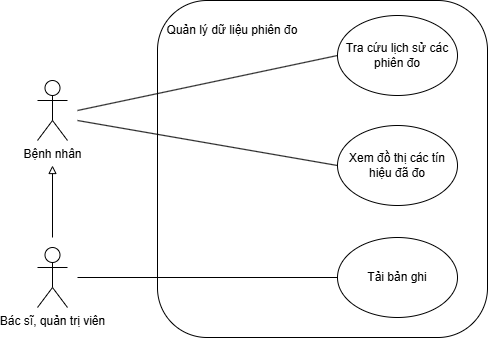
\includegraphics[width=12cm,height=10cm]{Images/use_case/use_case_record.png}
	\caption[Sơ đồ trường hợp sử dụng chức năng quản lý dữ liệu phiên đo]{\bfseries \fontsize{12pt}{0pt}
		\selectfont Sơ đồ trường hợp sử dụng chức năng quản lý dữ liệu phiên đo}
	\label{use_case_record} %đặt tên cho ảnh
\end{figure}

\begin{table}[H]
	\caption{\bfseries \fontsize{12pt}{0pt}\selectfont Phân tích trường hợp sử dụng chức năng tra cứu lịch sử các phiên đo}
	\centering
	\begin{tabularx}{0.9\textwidth}{|c|X|}
		\hline
		\textbf{Tên chức năng} & \textbf{Tra cứu lịch sử các phiên đo}                                                 \\
		\hline
		Tác nhân               & Người sử dụng hệ thống                                                                \\
		\hline
		Mô tả                  & Hỗ trợ người sử dụng hệ thống truy cập và quản lý lịch sử các phiên đo theo quyền hạn \\
		\hline
		Điều kiện trước        & Người dùng phải đăng nhập vào hệ thống                                                \\
		\hline
		Dòng sự kiện chính     &
		- Người dùng chọn tính năng xem lịch sử các phiên đo \newline
		- Hệ thống hiển thị danh sách dữ liệu các phiên đo dựa trên quyền hạn của người dùng: \newline
		+ Đối với bệnh nhân: Danh sách các phiên đo cá nhân \newline
		+ Đối với bác sĩ: Danh sách các phiên đo của bệnh nhân mà bác sĩ đang theo dõi \newline
		+ Đối với quản trị viên: Danh sách toàn bộ dữ liệu phiên đo trong hệ thống \newline
		- Hoàn thành quá trình tra cứu lịch sử các phiên đo                                                            \\
		\hline
	\end{tabularx}
\end{table}

\begin{table}[H]
	\caption{\bfseries \fontsize{12pt}{0pt}\selectfont Phân tích trường hợp sử dụng chức năng xem đồ thị các tín hiệu đã đo}
	\centering
	\begin{tabularx}{0.9\textwidth}{|c|X|}
		\hline
		\textbf{Tên chức năng} & \textbf{Xem đồ thị các tín hiệu đã đo}                                                                                           \\
		\hline
		Tác nhân               & Người dùng hệ thống (Bệnh nhân, Bác sĩ)                                                                                          \\
		\hline
		Mô tả                  & Hỗ trợ bệnh nhân và bác sĩ truy cập và xem đồ thị dữ liệu từ các phiên đo, cung cấp cái nhìn trực quan về các thông số tim mạch. \\
		\hline
		Điều kiện trước        & Người dùng cần đăng nhập vào hệ thống với quyền truy cập hợp lệ                                                                  \\
		\hline
		Dòng sự kiện chính     &
		- Người dùng truy cập chức năng xem đồ thị dữ liệu phiên đo \newline
		- Hệ thống hiển thị danh sách các phiên đo để người dùng lựa chọn \newline
		+ Đối với bệnh nhân: Danh sách các phiên đo cá nhân \newline
		+ Đối với bác sĩ: Danh sách các phiên đo của bệnh nhân mà bác sĩ đang theo dõi \newline
		+ Đối với quản trị viên: Danh sách toàn bộ dữ liệu phiên đo trong hệ thống \newline
		- Người dùng chọn một phiên đo cụ thể để xem đồ thị \newline
		- Hệ thống hiển thị đồ thị tương ứng dựa trên dữ liệu phiên đo đã chọn \newline
		- Hoàn thành quá trình xem đồ thị các tín hiệu đã đo                                                                                                      \\
		\hline
	\end{tabularx}
\end{table}

\begin{table}[H]
	\caption{\bfseries \fontsize{12pt}{0pt}\selectfont Phân tích trường hợp sử dụng chức năng tải bản ghi dữ liệu phiên đo}
	\centering
	\begin{tabularx}{0.9\textwidth}{|c|X|}
		\hline
		\textbf{Tên chức năng} & \textbf{Tải bản ghi dữ liệu phiên đo}                                                                                                                                                 \\
		\hline
		Tác nhân               & Bác sĩ, Quản trị viên                                                                                                                                                                 \\
		\hline
		Mô tả                  & Cung cấp chức năng tải về bản ghi dữ liệu phiên đo. Bác sĩ có thể tải dữ liệu từ bệnh nhân mà mình quản lý, trong khi quản trị viên có quyền tải về bất kỳ bản ghi nào trong hệ thống \\
		\hline
		Điều kiện trước        & Người dùng phải đăng nhập với quyền truy cập hợp lệ                                                                                                                                   \\
		\hline
		Dòng sự kiện chính     &
		- Người dùng truy cập chức năng tải bản ghi dữ liệu \newline
		- Hệ thống hiển thị danh sách các phiên đo khả dụng theo từng vai trò người dùng \newline
		- Người dùng chọn bản ghi cần tải xuống \newline
		- Hệ thống xử lý và trả về tệp dữ liệu phiên đo để tải xuống \newline
		- Tệp được tải thành công, hoàn thành quá trình tải bản ghi dữ liệu phiên đo                                                                                                                                   \\
		\hline
	\end{tabularx}
\end{table}

\begin{table}[H]
	\caption{\bfseries \fontsize{12pt}{0pt}\selectfont Phân tích trường hợp sử dụng chức năng phiên đo}
	\centering
	\begin{tabularx}{0.9\textwidth}{|c|X|}
		\hline
		\textbf{Tên chức năng} & \textbf{Xóa phiên đo}                               \\
		\hline
		Tác nhân               & Bác sĩ, Quản trị viên                               \\
		\hline
		Mô tả                  & Cung cấp chức năng xóa phiên đo.                    \\
		\hline
		Điều kiện trước        & Người dùng phải đăng nhập với quyền truy cập hợp lệ \\
		\hline
		Dòng sự kiện chính     &
		- Người dùng truy cập chức năng xóa dữ liệu phiên đo \newline
		- Hệ thống hiển thị danh sách các phiên đo có thể xóa \newline
		- Người dùng chọn phiên đo cần xóa dữ liệu \newline
		- Hệ thống thực hiện xóa phiên đo được chọn, cập nhật danh sách phiên đo và gửi thông báo kết quá \newline
		- Hoàn thành quá trình xóa dữ liệu phiên đo                                  \\
		\hline
	\end{tabularx}
\end{table}

\subsubsection{Sơ đồ trường hợp sử dụng chức năng quản lý dịch vụ lịch khám}

\begin{figure}[H]
	\centering
	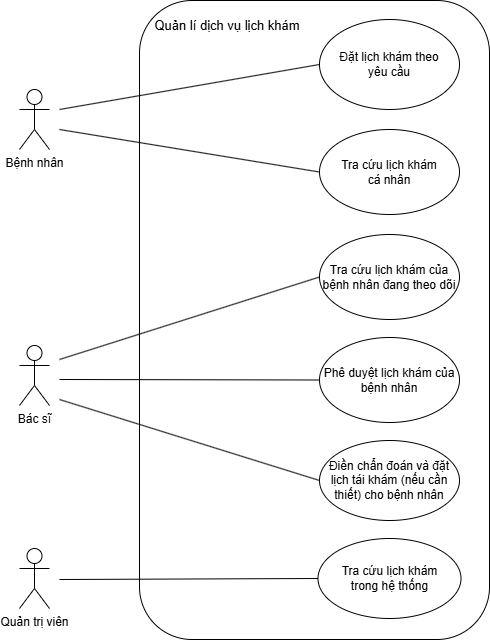
\includegraphics[width=12cm,height=15cm]{Images/use_case/use_case_schedule.png}
	\caption[Sơ đồ trường hợp sử dụng chức năng quản lý dịch vụ lịch khám]{\bfseries \fontsize{12pt}{0pt}
		\selectfont Sơ đồ trường hợp sử dụng chức năng quản lý dịch vụ lịch khám}
	\label{use_case_schedule} %đặt tên cho ảnh
\end{figure}

\begin{table}[H]
	\caption{\bfseries \fontsize{12pt}{0pt}\selectfont Phân tích trường hợp sử dụng chức năng đặt lịch khám theo yêu cầu}
	\centering
	\begin{tabularx}{0.9\textwidth}{|c|X|}
		\hline
		\textbf{Tên chức năng} & \textbf{Đặt lịch khám theo yêu cầu}                                                                                                                  \\
		\hline
		Tác nhân               & Bệnh nhân                                                                                                                                            \\
		\hline
		Mô tả                  & Cung cấp cho bệnh nhân khả năng linh hoạt trong việc đặt lịch khám, cho phép lựa chọn bác sĩ cụ thể hoặc thời gian rảnh phù hợp với nhu cầu cá nhân. \\
		\hline
		Điều kiện trước        & Bệnh nhân phải đăng nhập vào hệ thống với quyền truy cập hợp lệ                                                                                      \\
		\hline
		Dòng sự kiện chính     &
		- Bệnh nhân truy cập chức năng đặt lịch khám theo yêu cầu \newline
		- Hệ thống cung cấp hai lựa chọn: đặt lịch theo bác sĩ hoặc theo thời gian rảnh \newline
		+ Nếu đặt lịch theo bác sĩ: Hệ thống hiển thị danh sách bác sĩ và thời gian rảnh của từng bác sĩ để bệnh nhân lựa chọn \newline
		+ Nếu đặt lịch theo thời gian rảnh: Hệ thống hiển thị các khung thời gian trống và danh sách bác sĩ rảnh trong thời gian đó \newline
		- Bệnh nhân chọn thời gian và bác sĩ phù hợp để đặt lịch \newline
		- Hệ thống xử lý yêu cầu, lưu thông tin và thông báo đặt lịch thành công. Sau đó chờ lịch được xác nhận từ phía bác sĩ \newline
		- Hoàn thành quá trình đặt lịch                                                                                                                                               \\
		\hline
	\end{tabularx}
\end{table}

\begin{table}[H]
	\caption{\bfseries \fontsize{12pt}{0pt}\selectfont Phân tích trường hợp sử dụng chức năng tra cứu lịch khám trong hệ thống}
	\centering
	\begin{tabularx}{0.9\textwidth}{|c|X|}
		\hline
		\textbf{Tên chức năng} & \textbf{Tra cứu lịch khám trong hệ thống}                                           \\
		\hline
		Tác nhân               & Quản trị viên                                                                       \\
		\hline
		Mô tả                  & Cho phép quản trị viên xem và tra cứu chi tiết các lịch khám đang có trong hệ thống \\
		\hline
		Điều kiện trước        & Quản trị viên phải đăng nhập vào hệ thống với quyền truy cập hợp lệ                 \\
		\hline
		Dòng sự kiện chính     &
		- Quản trị viên truy cập chức năng tra cứu lịch khám \newline
		- Hệ thống hiển thị danh sách các lịch khám trong hệ thống \newline
		- Quản trị viên chọn một lịch khám cụ thể \newline
		- Hệ thống hiển thị chi tiết lịch khám, bao gồm thời gian, bác sĩ phụ trách, bệnh nhân và thông tin chẩn đoán (nếu có) \newline
		- Quá trình tra cứu lịch khám trong hệ thống hoàn tất                                                        \\
		\hline
	\end{tabularx}
\end{table}

\begin{table}[H]
	\caption{\bfseries \fontsize{12pt}{0pt}\selectfont Phân tích trường hợp sử dụng chức năng tra cứu lịch khám cá nhân}
	\centering
	\begin{tabularx}{0.9\textwidth}{|c|X|}
		\hline
		\textbf{Tên chức năng} & \textbf{Tra cứu lịch khám cá nhân}                                                                         \\
		\hline
		Tác nhân               & Bệnh nhân                                                                                                  \\
		\hline
		Mô tả                  & Cung cấp chức năng cho bệnh nhân dễ dàng tra cứu và xem thông tin chi tiết các lịch khám đã được chấp nhận \\
		\hline
		Điều kiện trước        & Bệnh nhân phải đăng nhập vào hệ thống với quyền truy cập hợp lệ                                            \\
		\hline
		Dòng sự kiện chính     &
		- Bệnh nhân truy cập chức năng tra cứu lịch khám cá nhân \newline
		- Hệ thống hiển thị danh sách các lịch khám của bệnh nhân đã được phê duyệt \newline
		- Bệnh nhân chọn một lịch khám cụ thể để xem thông tin chi tiết \newline
		- Hệ thống cung cấp thông tin chi tiết của lịch khám, bao gồm thời gian, bác sĩ phụ trách và chẩn đoán nếu có \newline
		- Quá trình tra cứu lịch khám cá nhân hoàn tất                                                                                      \\
		\hline
	\end{tabularx}
\end{table}

\begin{table}[H]
	\caption{\bfseries \fontsize{12pt}{0pt}\selectfont Phân tích trường hợp sử dụng chức năng tra cứu lịch khám của bệnh nhân đang được theo dõi}
	\centering
	\begin{tabularx}{0.9\textwidth}{|c|X|}
		\hline
		\textbf{Tên chức năng} & \textbf{Tra cứu lịch khám của bệnh nhân đang được theo dõi}                                                 \\
		\hline
		Tác nhân               & Bác sĩ                                                                                                      \\
		\hline
		Mô tả                  & Cho phép bác sĩ tra cứu danh sách và xem thông tin chi tiết các lịch khám của bệnh nhân mà bác sĩ phụ trách \\
		\hline
		Điều kiện trước        & Bác sĩ phải đăng nhập vào hệ thống với quyền truy cập hợp lệ                                                \\
		\hline
		Dòng sự kiện chính     &
		- Bác sĩ truy cập chức năng tra cứu lịch khám của bệnh nhân đang được theo dõi \newline
		- Hệ thống hiển thị danh sách các lịch khám đã được đặt (cả thành công và đang chờ xét duyệt) \newline
		- Bác sĩ chọn một lịch khám cụ thể để xem thông tin chi tiết \newline
		- Hệ thống cung cấp thông tin chi tiết của lịch khám, bao gồm thời gian, bệnh nhân đặt lịch và chẩn đoán nếu có \newline
		- Quá trình tra cứu lịch khám của bệnh nhân đang được theo dõi hoàn tất                                                              \\
		\hline
	\end{tabularx}
\end{table}

\begin{table}[H]
	\caption{\bfseries \fontsize{12pt}{0pt}\selectfont Phân tích trường hợp sử dụng chức năng phê duyệt lịch khám}
	\centering
	\begin{tabularx}{0.9\textwidth}{|c|X|}
		\hline
		\textbf{Tên chức năng} & \textbf{Phê duyệt lịch khám của bệnh nhân}                                                                           \\
		\hline
		Tác nhân               & Bác sĩ                                                                                                               \\
		\hline
		Mô tả                  & Cung cấp chức năng cho bác sĩ phê duyệt lịch khám của bệnh nhân, bao gồm chấp nhận hoặc từ chối các yêu cầu đặt lịch \\
		\hline
		Điều kiện trước        & Bác sĩ phải đăng nhập vào hệ thống với quyền truy cập hợp lệ                                                         \\
		\hline
		Dòng sự kiện chính     &
		- Bác sĩ truy cập chức năng phê duyệt lịch khám của bệnh nhân đã đặt \newline
		- Hệ thống hiển thị danh sách các lịch khám đang chờ phê duyệt \newline
		- Bác sĩ chọn một lịch khám cụ thể để xem chi tiết thông tin \newline
		- Bác sĩ thực hiện chấp nhận hoặc từ chối yêu cầu đặt lịch \newline
		- Nếu chấp nhận: Hệ thống cập nhật trạng thái lịch khám thành "Đã phê duyệt" và thông báo cho bệnh nhân \newline
		- Nếu từ chối: Hệ thống yêu cầu bác sĩ xác nhận và cung cấp lý do từ chối, sau đó thông báo cho bệnh nhân \newline
		- Quá trình phê duyệt lịch khám hoàn tất                                                                                                      \\
		\hline
	\end{tabularx}
\end{table}

\begin{table}[H]
	\caption{\bfseries \fontsize{12pt}{0pt}\selectfont Phân tích trường hợp sử dụng chức năng điền chẩn đoán và đặt lịch tái khám}
	\centering
	\begin{tabularx}{0.9\textwidth}{|c|X|}
		\hline
		\textbf{Tên chức năng} & \textbf{Điền chẩn đoán và đặt lịch tái khám}                                                 \\
		\hline
		Tác nhân               & Bác sĩ                                                                                       \\
		\hline
		Mô tả                  & Hỗ trợ bác sĩ điền thông tin chẩn đoán cho từng lịch khám và đặt lịch tái khám nếu cần thiết \\
		\hline
		Điều kiện trước        & Bác sĩ phải đăng nhập vào hệ thống với quyền truy cập hợp lệ                                 \\
		\hline
		Dòng sự kiện chính     &
		- Bác sĩ truy cập chức năng điền chẩn đoán \newline
		- Chọn lịch khám cần điền hoặc cập nhật chẩn đoán \newline
		- Hệ thống hiển thị chi tiết lịch khám đã chọn \newline
		- Bác sĩ điền hoặc cập nhật thông tin chẩn đoán \newline
		- Nếu cần tái khám, bác sĩ nhấn nút "Đặt lịch tái khám" và nhập thời gian phù hợp \newline
		- Hệ thống lưu thông tin và hoàn tất quy trình                                                                        \\
		\hline
	\end{tabularx}
\end{table}

\subsubsection{Sơ đồ trường hợp sử dụng chức năng quản lý dịch vụ nhắn tin}

\begin{figure}[H]
	\centering
	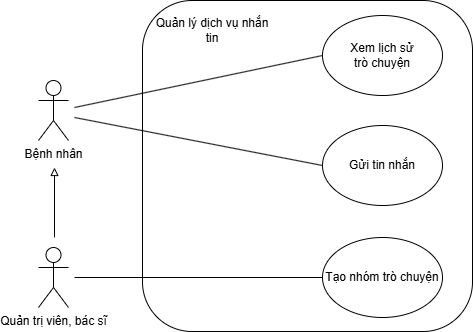
\includegraphics[width=12cm,height=9cm]{Images/use_case/use_case_chat.png}
	\caption[Sơ đồ trường hợp sử dụng chức năng quản lý dịch vụ nhắn tin]{\bfseries \fontsize{12pt}{0pt}
		\selectfont Sơ đồ trường hợp sử dụng chức năng quản lý dịch vụ nhắn tin}
	\label{use_case_chat} %đặt tên cho ảnh
\end{figure}

\begin{table}[H]
	\caption{\bfseries \fontsize{12pt}{0pt}\selectfont Phân tích trường hợp sử dụng chức năng xem lịch sử trò chuyện}
	\centering
	\begin{tabularx}{0.9\textwidth}{|c|X|}
		\hline
		\textbf{Tên chức năng} & \textbf{Xem lịch sử trò chuyện}                                                              \\
		\hline
		Tác nhân               & Người sử dụng hệ thống                                                                       \\
		\hline
		Mô tả                  & Cung cấp cho người dùng khả năng truy cập và xem lại lịch sử các đoạn hội thoại đã thực hiện \\
		\hline
		Điều kiện trước        & Người dùng phải đăng nhập vào hệ thống với quyền truy cập hợp lệ                             \\
		\hline
		Dòng sự kiện chính     &
		- Người dùng truy cập chức năng nhắn tin và chọn đoạn hội thoại mong muốn \newline
		- Hệ thống hiển thị nội dung chi tiết của đoạn hội thoại đã chọn \newline
		- Hoàn thành quá trình xem lịch sử trò chuyện                                                                         \\
		\hline
	\end{tabularx}
\end{table}

\begin{table}[H]
	\caption{\bfseries \fontsize{12pt}{0pt}\selectfont Phân tích trường hợp sử dụng chức năng gửi tin nhắn}
	\centering
	\begin{tabularx}{0.9\textwidth}{|c|X|}
		\hline
		\textbf{Tên chức năng} & \textbf{Gửi tin nhắn}                                                                                                                                                                                                                                       \\
		\hline
		Tác nhân               & Người sử dụng hệ thống                                                                                                                                                                                                                                      \\
		\hline
		Mô tả                  & Cung cấp chức năng cho phép người dùng gửi tin nhắn đến các đối tượng liên quan: bác sĩ chỉ gửi tin nhắn được với quản trị viên và những bệnh nhân mình theo dõi. Tương tự, bệnh nhân cũng chỉ gửi được tin nhắn cho bác sĩ đã chấp nhận lịch khám của mình \\
		\hline
		Điều kiện trước        & Người dùng phải đăng nhập với quyền truy cập hợp lệ                                                                                                                                                                                                         \\
		\hline
		Dòng sự kiện chính     &
		- Người dùng truy cập chức năng gửi tin nhắn \newline
		- Chọn người nhận hoặc nhóm nhận tin nhắn \newline
		- Hệ thống hiển thị biểu mẫu để nhập nội dung tin nhắn \newline
		- Người dùng nhập nội dung và nhấn nút gửi \newline
		- Hệ thống gửi tin nhắn đến người nhận hoặc nhóm và thông báo thành công \newline
		- Hoàn thành quá trình gửi tin nhắn                                                                                                                                                                                                                                                  \\
		\hline
	\end{tabularx}
\end{table}

\begin{table}[H]
	\caption{\bfseries \fontsize{12pt}{0pt}\selectfont Phân tích trường hợp sử dụng chức năng tạo nhóm trò chuyện}
	\centering
	\begin{tabularx}{0.9\textwidth}{|c|X|}
		\hline
		\textbf{Tên chức năng} & \textbf{Tạo nhóm trò chuyện}                                                      \\
		\hline
		Tác nhân               & Quản trị viên, Bác sĩ                                                             \\
		\hline
		Mô tả                  & Cho phép người dùng tạo nhóm trò chuyện để trao đổi thông tin giữa các thành viên \\
		\hline
		Điều kiện trước        & Người dùng phải đăng nhập với quyền truy cập hợp lệ                               \\
		\hline
		Dòng sự kiện chính     &
		- Người dùng truy cập chức năng tạo nhóm trò chuyện \newline
		- Hệ thống hiển thị biểu mẫu tạo nhóm \newline
		- Người dùng nhập thông tin nhóm và thêm thành viên vào nhóm \newline
		- Hệ thống tạo nhóm thành công và gửi thông báo đến các thành viên \newline
		- Hoàn thành quá trình tạo nhóm trò chuyện                                                                 \\
		\hline
	\end{tabularx}
\end{table}

\newpage